\newpage
\section{H�here und strukturierte Datentypen}
	\begin{minipage}[t]{6 cm} 		
  		\subsection{Pointer}
  			Pointer sind in \lc{C++} zu 99\% wie in \lc{C}. \\
		\subsubsection{Null-Pointer}
			Ab \lc{C++11} gibt es einen vordefinierten Wert f�r den Nullpointer: \lc{nullptr}
			\vspace*{-0.2cm}\lstinputlisting{code/pointer_null.c}
	\end{minipage}	
	\hspace*{0.5cm}
	\begin{minipage}[t]{12 cm}
		\subsubsection{$void$-Pointer}
			\begin{compactitem}
				\item Wenn bei der Definition des Pointers der Typ der Variable, auf die der Pointer zeigen soll, noch nicht feststeht, wird ein Pointer auf den Typ \lc{void} vereinbart.
				\item Ein Pointer auf \lc{void} umgeht die Typenpr�fung des Compilers. Er kann ohne \lc{typecast} einem typisierten Pointer zugewiesen werden aber er kann keine Zuweisung von einem typisierten Pointer erhalten (in \lc{C} erlaubt).
				\item Jeder Pointer kann durch Zuweisung in den Typ \lc{void*} und zur�ck umgewandelt werden, ohne dass Informationen verloren gehen.
			\end{compactitem}
 	\end{minipage}
 	       
	\subsubsection{Pointer auf Funktionen}
		\begin{minipage}[t]{10 cm}
			\vspace*{-0.5cm}\lstinputlisting{code/pointer_funktion.c}
		\end{minipage}
		\hspace*{0.5cm}
		\begin{minipage}[t]{8 cm}
			\vspace*{-0.6cm}
			\textbf{Vereinbarung eines Pointers}
				\lstinputlisting{code/pointer_funktion_vereinbarung.c}
				$ptr$ ist hier ein pointer auf eine Funktion mit R�ckgabewert vom Typ $int$ und einem �bergabeparameter vom Typ $char$. Die Klammern m�ssen unbedingt gesetzt werden. \\
			
			\textbf{Zuweisung einer Funktion}
				\lstinputlisting{code/pointer_funktion_zuweisung.c} \ \\
				
			\vspace*{-0.7cm}\textbf{Aufruf einer Funktion}
				\lstinputlisting{code/pointer_funktion_aufruf.c}
		\end{minipage}
       
	\subsubsection{const bei Pointern}
		\vspace*{-0.3cm}
		\begin{minipage}[t]{5 cm}
			\paragraph{konstanter String}
			\vspace{-0.5cm}
			\lstinputlisting{code/const_pointer_1.c}
		\end{minipage}
		\hspace*{0.5cm}
		\begin{minipage}[t]{5 cm}
			\paragraph{konstanter Pointer}
			\vspace{-0.5cm}
				\lstinputlisting{code/const_pointer_2.c}
		\end{minipage} 
		\hspace*{0.5cm}
		\begin{minipage}[t]{7.5 cm}					
			\paragraph{konst. Pointer auf konst. String}
				\vspace{-0.5cm}
				\lstinputlisting{code/const_pointer_3.c}
		\end{minipage} 

\phantom{}

	\subsection{Referenzen}
		\begin{compactitem}
			\item Referenzen sind alternative Namen oder Alias f�r ein Objekt
			\item Beim Pointer m�chte man eine Adresse, eine Referenz kann auch auf Register verweisen
			\item Wenn immer m�glich sollten Referenzen verwendet werden, weil sicherer
		\end{compactitem}
		\begin{minipage}[t]{10.5 cm}
	  		\vspace*{-0.3cm}\lstinputlisting{code/ref1.c}
	  	\end{minipage}				
   
	\subsection{Pointer und Referenzen als R�ckgabewert und Parameter�bergabe}
  		Bei Variablen�bergabe (call by value) werden Kopien �bergeben, welche nicht ver�ndert werden k�nnen.\\
  		Bei Referenz�bergabe (call by reference) kann die Subroutine die Werte bleibend ver�ndern. \\
  		\textbf{Objekte einer Klasse und Strukturvariablen sollen immer by reference �bergeben werden!} \\
  		\begin{minipage}[t]{5.5 cm}
  			\subsubsection{call by reference}
   				\lstinputlisting{code/swap.c} 
   		\end{minipage}
   		\hspace*{0.5cm}
    	\begin{minipage}[t]{5.5 cm}
      			\vspace*{0.77cm} \lstinputlisting{code/swap2.c} 
      	\end{minipage}
      	\hspace*{0.5cm}
      	\begin{minipage}[t]{6 cm}
      		\subsubsection{call by value}
      	      	\lstinputlisting{code/swap3.c} 
      	\end{minipage}
      \\
      
    \subsection{Dynamische Speicherverwaltung}
    	\begin{minipage}[t]{9 cm}
    		\subsubsection{pro Memoria: Variablen}
	    		\begin{compactitem}
	    			\item erleichtern u.a. den Zugriff auf Speicherstellen (anstelle Adressen)
	    			\item M�ssen zur Entwicklungszeit im Code definiert werden
	    			\item Der Speicher einer Variable wird automatisch freigegeben, sobald die Variable nicht mehr g�ltig ist.
	    		\end{compactitem}  	
	    	\subsubsection{Dynamische Speicherverwaltung}
		    	\begin{compactitem}
		    		\item Speicher kann zur Laufzeit (dynamisch) vom System angefordert (alloziert) werden
		    		\begin{compactitem} \item Operator: $new$ (in $C$: Funktion $malloc()$) \end{compactitem}
		    		\item Dynamisch allozierter Speicher muss wieder explizit freigegeben werden
		    		\begin{compactitem} \item Operator: $delete$ (in $C$: Funktion $free()$) \end{compactitem}
		    		\item Dynamischer Speicher wird nicht auf dem Stack angelegt, sondern auf dem {\bf Heap}
		    		\item Auf Dynamisch allozierter Speicher kann {\bf nur} �ber Pointer zugegriffen werden
		    	\end{compactitem}
	    \end{minipage}
		\hspace*{0.5cm}
		\begin{minipage}[t]{9 cm}
			\subsubsection{Syntax}
			\vspace*{-0.3cm}
			\lstinputlisting{code/speicherverw.c}
		\end{minipage}
	
	\subsubsection{Vorsichtsmassnahmen}
		\begin{compactitem}
			\item Beim Anwenden des delete-Operator auf einen bereits freigegebenen Speicherbereich, kann Probleme verursachen.
			\item Oft wird deshalb ein Pointer nach der $delete$-Operation auf 0 (bzw. $nullptr$) gesetzt.
		\end{compactitem}
	
	\subsubsection{Memory Leak, Garbage Collection}
	\begin{compactitem}
		\item {\bf Memory Leak} = Speicher, der nicht freigegeben wurde oder auf welchen der Zugriff verloren ging, belegt
		aber weiterhin Platz im Speicher. (wie ein Leck)
		\item In einigen Programmiersprachen (wie z.B. Java) gibt es einen sogenannten {\bf Garbage Collector}, welcher dieser Speicher automatisch freigibt.
		\item In C++ gibt es keinen Garbage Collector. Der Programmierer ist selber daf�r verantwortlich.
	\end{compactitem}
 		
	\subsubsection{Dynamische Allozierung von Arrays}
		\begin{minipage}[t]{7 cm} 
			\begin{compactitem}
				\item mit \lc{new[]} kann dynamischer Speicher f�r ein Array alloziert werden.
				\item Zugriff erfolgt wie bei statischen Arrays.
				\item Mit \lc{delete[]} k�nnen dynamisch allozierte Arrays wieder explizit freigegeben werden.
			\end{compactitem}
		\end{minipage}
		\hspace*{0.5cm}
		\begin{minipage}[t]{11 cm}
			\vspace*{-0.3cm}
			\lstinputlisting{code/vec2.c}
		\end{minipage}
	
	\subsubsection{Dynamische Allozierung von Matrizen}
		\paragraph{Variante 1}
			\begin{compactitem}
				\item m*n-Matrix als eindimensionaler Array der Gr�sse (m*n)
				\item Zugriff nur �ber Pointer:
			\end{compactitem}
			\lstinputlisting{code/matrix1.cpp}
    	\paragraph{Variante 2}
    		\begin{compactitem}
				\item Ein Array der Gr�sse m und dem Typ Array
				\item Auf ein Matrixelement kann somit �ber Arrayindizes zugegriffen werden:
    		\end{compactitem}
    		\lstinputlisting{code/matrix2.cpp}
    		\begin{minipage}[t]{9 cm}
    			\vspace*{-2.5 cm}
    			\lstinputlisting{code/matrix3.cpp}
    		\end{minipage}
    		\hspace*{0.5cm}
    		\begin{minipage}[t]{9 cm}
    			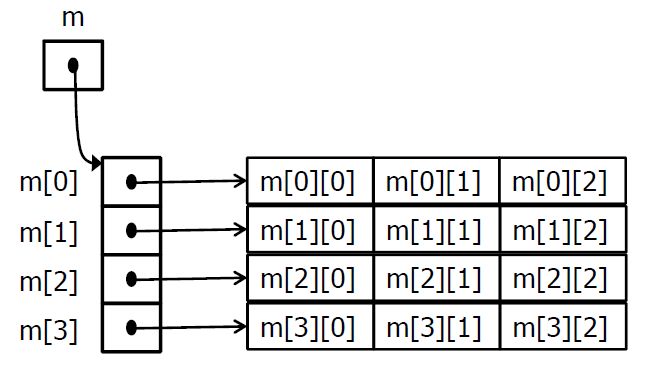
\includegraphics[width=5cm]{pics/matrix.png}
    		\end{minipage}
    		\begin{compactitem}
    			\item Jedes \lc{m[i]} ist ein Pointer auf ein Array mit 3 Elementen vom Typ \lc{double}.
    			\item \lc{m[i]} selbst ist vom Typ \lc{double*}.
    			\item der Speicher von Matrizen wird wie folgt freigegeben (zuerst jede Zeile dann Array mit \lc{double*}):
			\end{compactitem}
			\lstinputlisting{code/matrixDel.cpp}
		\paragraph{Vor- und Nachteile Variante 2}
			\begin{compactitem}
				\vspace*{-0.3cm}
				\item Nur mit der Variante 2 kann �ber Arrayindizes zugegriffen werden
				\item Die einzelnen Zeilen liegen m�gicherweise nicht auf aufeinanderfolgenden Speicherstellen
				\item Der Zugriff ist effizienter, obwohl man zus�tzliche Pointer ben�tigt
			\end{compactitem}
			
	\subsection{Structs}
		\begin{minipage}[t]{5 cm}
			\begin{compactitem}
				\item Grunds�tlich wie in $C$
				\item $typedef$ braucht es nicht
			\end{compactitem}	
		\end{minipage}
		\hspace*{0.5cm}
		\begin{minipage}[t]{5 cm}
			{\bf Beispiel in $C$:}
			\lstinputlisting{code/structC.c}
		\end{minipage}  
		\hspace*{0.5cm}
		\begin{minipage}[t]{5 cm}
		{\bf Beispiel in $CPP$:}
		\lstinputlisting{code/structCpp.cpp}
		\end{minipage} 
		
